\chapter{Thread}
\thispagestyle{empty}

Nei sistemi operativi tradizionali ogni processo ha uno spazio di indirizzamento e un singolo \textbf{thread} di controllo. Ci sono tuttavia situazioni in cui è desiderabile avere molti thread di controllo nello stesso spazio di indirizzamento, in esecuzione in parallelo come se fossero processi separati.

\section{Il modello a thread}
Il modello a processi visto finora è basato su due concetti indipendenti tra loro: raggruppamento delle risorse ed esecuzione. Qualche volta è utile separarli, ed è qui che entrano in gioco i thread.

Un concetto che un processo racchiude è quello di thread di esecuzione, normalmente abbreviato con thread. Il \textit{thread} ha un program counter che tiene traccia della prossima istruzione da eseguire, ha dei registri, uno stack\dots

I processi sono usati per raggruppare le risorse, i thread invece sono le entità schedulate per l'esecuzione nella CPU.
Quello che i thread aggiungono al modello a processi è il permettere molte esecuzioni nell'ambiente di un processo, indipendenti l'una dall'altra.

Poiché i thread hanno solo alcune proprietà dei processi vengono a volte chiamati \textit{processi leggeri}. Il termine \textbf{multithreading} è usato per descrivere quella situazione in cui ad un processo sono assegnati più thread.

\begin{figure}[H]
    \centering
    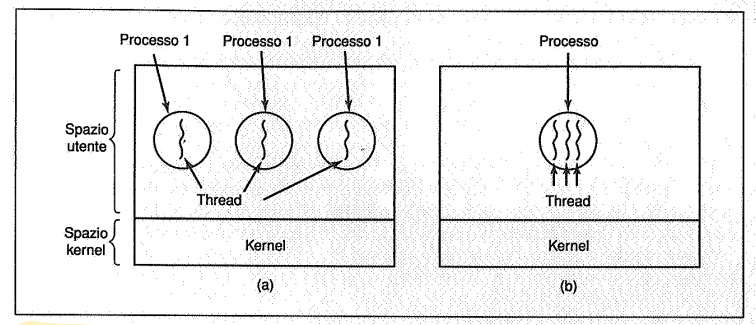
\includegraphics[width=0.9\linewidth]{assets/multi5.png}
    \caption{ }
    \label{multi5}
\end{figure}

In entrambi i casi presentati dalla figura \ref{multi5} abbiamo tre thread, nel primo caso ciascuno opera in uno spazio di indirizzamento diverso dagli altri, nel secondo caso lo spazio è condiviso. COnviene utilizzare la seconda soluzione nel caso in cui i thread sono veramente parte dello stesso job e cooperano l'un l'altro attivamente.

Quando un processo con thread multipli viene eseguito la CPU passa rapidamente tra uno a l'altro, dando l'impressione di un esecuzione parallela.

Rispetto che per i processi, per i thread non esiste protezione, non è necessaria e sarebbe comunque impossibile da realizzare.

Oltre che lo stesso spazio di indirizzamento i thread condividono: lo stesso insieme di file aperti, processi figli, allarmi, segnali\dots

\begin{figure}[H]
    \centering
    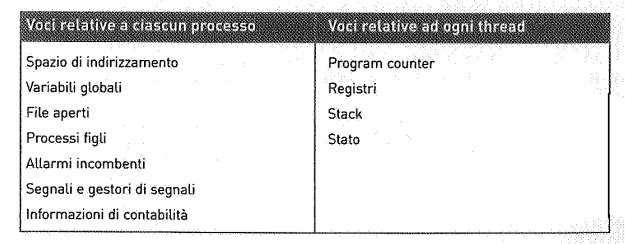
\includegraphics[width=0.9\linewidth]{assets/risorse5.png}
    \caption{ }
\end{figure}


Come un processo tradizionale (ovvero dotato di un singolo thread) anche i thread possono trovarsi in uno qualsiasi dei diversi stati: pronto, esecuzione, bloccato, terminato. Vale la stessa cosa per le transizioni degli stati, sono analoghe a quelle dei processi.

È importante capire che ogni thread ha il proprio stack, esso contiene un elemento per ogni procedura chiamata non ancora conclusa, con le variabili locali della procedura e gli indirizzi di ritorno. Ogni thread chiamerà generalmente procedure diverse ed avrà quindi una diversa storia di esecuzione.

Quando è presente \textit{multithreading} normalmente i processi partono con un solo thread, che ha la capacità di creare nuovi thread con una procedura di libreria, ad esempio \textbf{thread\_create}, con un parametro indicante una procedura che il nuovo thread deve eseguire.

Qualche volta i thread sono gerarchici, altre volte essi sono equivalenti tra loro. In entrambi i casi ad un thread che ne crea un altro viene restituito un identificatore di quest'ultimo.

Quando un thread ha finito chiama un'altra procedura di libreria, la \textbf{thread\_exit}. In alcuni sistemi è possibile che un thread aspetti che uno specifico thread termini con la chiamata di procedura \textbf{thread\_wait}.

Un'altra chiamata comune è la \textbf{thread\_yield} che permette di cedere la CPU ad un altro thread, perché venga eseguito. È una chiamata importante in quanto non esiste un interruzione di clock per realizzare il desiderato timesharing.

Oltre a vantaggi i thread introducono anche delle complicazioni.. che fare quando un \textit{processo} genitore ha thread multipli e chiama la \textit{fork()}? Se il figlio ottiene tanti thread quanti il genitore che succede se un thread del genitore viene bloccato?

O ancora, che succede se un thread che condivide file aperti con altri chiude un file che un altro stava ancora leggendo?

Occorre prestare molta attenzione a come programmare i diversi compiti di ciascun thread.

\section{Uso dei thread}
I/O
I thread possono essere creati e distrutti più facilmente dei processi, poiché non hanno alcuna risorsa associata.
Essi non portano alcun guadagno quando sono tutti \textit{CPU bound}, quando invece sono presenti molte operazioni \textit{I/O} danno il loro meglio.

I thread sono utili anche per sistemi con CPU multiple, in cui è possibile un reale parallelismo.

Come esempio si può considerare un elaboratore di testo: utilizzando tre thread il modello di programmazione è molto più semplice, il primo può occuparsi dell'interazione con l'utente, il secondo della riformattazione del documento e il terzo che salva il contenuto della RAM su disco periodicamente. Si noti che avere tre processi che operano separatamente in questo caso non funzionerebbe.

In generale, in informatica, quando in un modello ogni computazione ha uno stato salvato ed esistono un insieme di eventi per permettere il cambio di stato, si parla di \textbf{macchina a stati finiti}.

Ciò che offrono i thread quindi è parallelismo anche in quei casi in cui l'idea del processo è sequenziale con chiamate di sistema bloccanti.

\section{Implementazione dei thread}

Ci sono due modi principali di implementare i thread: nello spazio utente e nel kernel.

\begin{figure}[H]
    \centering
    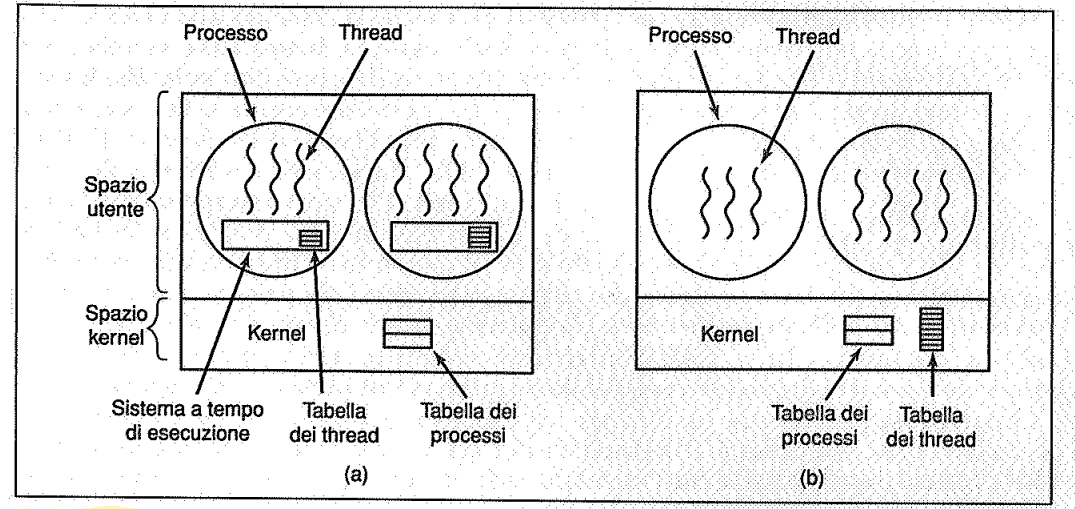
\includegraphics[width=0.9\linewidth]{assets/impl5.png}
    \caption{(a) thread package a livello utente. (b) thread package gestito dal kernel.}
    \label{impl5}
\end{figure}

\subsection{Nello spazio utente}

In questo metodo i thread sono completamente nello spazio utente, il kernel non sa nulla di loro e gestirà i processi ordinari ad un solo thread.

Il primo vantaggio di questa soluzione è permettere l'implementazione dei thread anche in quei sistemi operativi che non li supportano nativamente.

Come si vede in figura \ref{impl5}(a) i thread sono eseguiti sopra ad un sistema a tempo di esecuzione, ovvero una collezione di procedure che li gestiscono.

In questa soluzione ogni processo ha bisogno della propria \textbf{tabella dei thread}, analoga a quella dei processi. Anch'essa è gestita dal sistema a tempo di esecuzione.

Quando un thread fa qualcosa che potrebbe bloccarlo localmente chiama una procedura a tempo di esecuzione, la quale controlla se il thread va effettivamente bloccato. In caso affermativo essa salva le informazioni utili nella tabella dei thread e ricarica i registri macchina con i valori salvati del nuovo thread. Non appena SP e PC vengono aggiornati parte l'esecuzione di quello nuovo senza la necessità di altre operazioni.

Scambiare thread in questo modo è almeno un ordine di grandezza più rapido che usare le trap del kernel, questo è un grande vantaggi dell'implementazione nello spazio utente.
Esiste infatti una differenza chiave con i processi, la procedura che salva lo stato dei thread e lo schedulatore sono procedure locali, invocarle è quindi molto più efficiente che chiamare in causa il kernel.

Altri vantaggi di questo metodo sono: ogni processo può avere il proprio algoritmo di schedulazione, migliore scalabilità (rispetto a quelli implementati nel kernel non hanno bisogno di spazio per tabelle e stack direttamente nel kernel).

Uno degli svantaggi invece è l'implementazione delle chiamate di sistema bloccanti: se un thread legge da tastiera prima che un tasto sia premuto è impensabile lasciare che il thread esegua effettivamente la chiamata di sistema, bloccherebbe tutti i thread.

Nota: in alcune versioni UNIX esiste una scappatoia al problema: la chiamata di sistema \textbf{select} che permette di dire se una chiamata si bloccherà, prima di eseguirla. Nel caso si usi questa soluzione il codice intorno alla vera chiamata di sistema (che quindi effettuerà la \textit{select}) è chiamato \textbf{wrapper}.

Un altro problema analogo è quello del \textit{fault} di pagina, esso si verifica quando un thread fa un salto ad un area di memoria non caricata in RAM, in quel caso il sistema operativo blocca tutto per andare a caricare in RAM la porzione richiesta, compresi i thread che non c'entrano nulla, in quanto non ne conosce l'esistenza.

Un ultimo problema si ha nella gestione stessa: quando un thread inizia l'esecuzione nessun altro thread in quel processo verrà eseguito, a meno che il primo non rilasci spontaneamente la CPU. Se un thread non entra nel sistema a tempo di esecuzione lo schedulatore non piò far nulla.


La gestione dei thread a livello utente è fatta tramite librerie:
\begin{itemize}
    \item POSIX Pthreads
    \item Java threads
    \item C-threads (Mach)
    \item API di win32
\end{itemize}

Un semplice programma che usa la libreria Pthreads:
\lstinputlisting{code/chap5.c}

\subsection{Nel kernel}

Se il kernel conosce e gestisce i thread non serve un sistema a tempo di esecuzione. Questa situazione è mostrata in figura \ref{impl5}(b). Non c'è una tabella dei thread per ogni processo ma ne esiste una globale.

Quando un thread vuole ne vuole creare un altro esso esegue una chiamata di sistema che aggiornerà la tabella dei thread. La tabella conterrà le stesse informazioni di prima ma sarà salvata nel kernel.

Tutte le chiamate che possono bloccare un thread sono chiamate di sistema, hanno quindi un costo decisamente più elevato, tuttavia il kernel può decidere di far continuare l'esecuzione di un altro thread appartenente al processo (oppure di un altro processo) nel frattempo che il thread risulta bloccato.

Per sopperire un po' all'eccessivo costo di creazione e distruzione dei thread alcuni sistemi implementano strategie ad hoc che consistono nel riciclaggio dei thread, questo permette di ridurre il grande \textit{overhead} causato dal problema.

Esiste un problema aggiuntivo e riguarda la schedulazione: se il processo A ha 1 thread ed il processo B ne ha 100, se implementati a livello utente i thread di B ottengono un centesimo del tempo di CPU del thread di A, se invece vengono implementati nel kernel a ciascun thread viene assegnato lo stesso tempo di CPU, ma a questo punto il processo A ottiene un centesimo rispetto al processo B\dots

\section{Programmazione multithread}

Esistono diversi approcci nella programmazione multithread:
\begin{itemize}
    \item \textbf{molti a uno}: in questo caso molti thread a livello utente sono mappati in un singolo thread del nucleo. [\textit{solaris green thread} e \textit{GNU portable thread}]
    \item \textbf{uno a uno}: ad ogni thread a livello utente ne corrisponde uno nel nucleo. [\textit{windows NT/XP/2000}, \textit{linux}, \textit{solaris 9+}]
    \item \textbf{molti a molti}: molti thread a livello utente mappati in molti thread nel kernel. Permette al sistema operativo di creare un numero sufficiente di thread a livello del nucleo. [\textit{solaris 9-}, \textit{windows NT/2000(lib. ThreadFIber)}]
    \item \textbf{a due livelli}: simile al molti-a-molti ma permette ad un thread utente di essere associato ad un thread del nucleo. [\textit{irix}, \textit{hp-ux}, \textit{tru64 unix}, \textit{solaris 8-}]
\end{itemize}

\begin{figure}[H]
    \centering 
    \subfloat[molti a uno]{%
      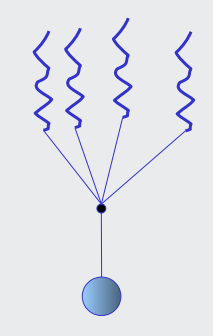
\includegraphics[width=0.2\linewidth]{assets/moltiuno5.png}%
    }\qquad
%
    \subfloat[uno a uno]{%
      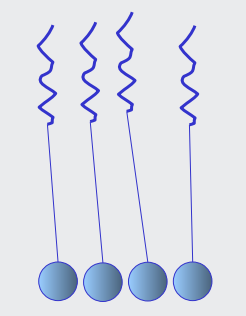
\includegraphics[width=0.2\linewidth]{assets/unouno5.png}%
    }\qquad
%
    \subfloat[molti a molti]{%
      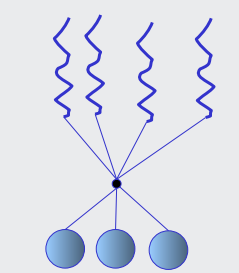
\includegraphics[width=0.2\linewidth]{assets/moltimolti5.png}%
    }\qquad
%
    \subfloat[a due livelli]{%
      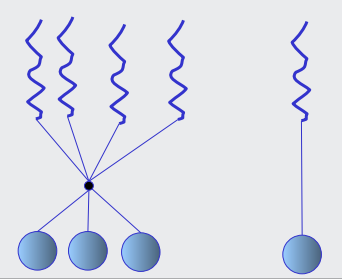
\includegraphics[width=0.2\linewidth]{assets/duelivelli5.png}%
    }
%
    \caption{ }
  \end{figure}

\section{Unix}
I segnali in UNIX sono usati per comunicare ad un processo il verificarsi di un particolare evento. 

Lo schema si ripete:
\begin{enumerate}
  \item il segnale viene generato da un evento.
  \item il segnale viene inviato ad un processo.
  \item il segnale viene gestito: 
        \begin{itemize}
          \item viene inviato al thread a cui si riferisce.
          \item ogni thread riceve lo riceve.
          \item solo alcuni thread lo ricevono.
          \item esiste un unico thread che li gestisce tutti.
        \end{itemize}
\end{enumerate}

Nota che nella terminologia Linux si parla di \textbf{task} invece che thread. La loro creazione avviene tramite la chiamata di sistema \textit{clone()}, che permette al task figlio di condividere lo spazio di indirizzi del task genitore. La \textit{fork()} diventa allora solo un caso particolare della \textit{clone()}.

\section{I thread di java}

\dots